\documentclass{article}
\usepackage[headheight=40pt, textheight=560pt]{geometry}
\usepackage{paralist}
\usepackage{scalerel,amssymb}
\usepackage{amsmath}
\usepackage{colortbl}
\usepackage{array}
\usepackage{multirow}
\usepackage{blindtext}
\usepackage{reledmac}
\usepackage{changepage}

\usepackage{pgfplots}
\usepackage{tikz}
\usetikzlibrary{positioning}
\usetikzlibrary{shapes.geometric, arrows}
\tikzstyle{arrow} = [thick,->,>=stealth]

\usepackage{graphicx}
\usepackage{stix}

\newcommand{\tableflip}{$($\rotatebox{45}{$\smile$}$^{\circ}\smwhtsquare^{\circ})\rotatebox{45}{$\smile$}\mkern-6mu\frown$\raisebox{0.5ex}{$\bot$}$\mkern-3.5mu-\mkern-3.5mu$\raisebox{0.5ex}{$\bot$}}

\usepackage{stackengine}
\def\apeqA{\SavedStyle\sim}
\def\apeq{\setstackgap{L}{\dimexpr.5pt+1.5\LMpt}\ensurestackMath{%
  \ThisStyle{\mathrel{\Centerstack{{\apeqA} {\apeqA} {\apeqA}}}}}}

\usepackage{fancyhdr}
\fancyhead[L]{
	\begin{tabular}{ll}
		\begin{tabular}{l}
			%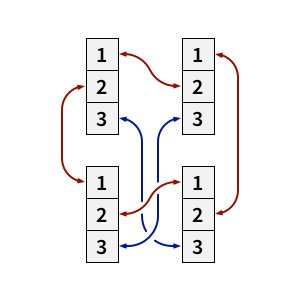
\includegraphics[scale=0.13]{distributed}
		\end{tabular}	
		&
		\begin{tabular}{l}
			\LARGE \textbf{Wirtschaftsinformatik} \\
			\Large \textsc{Zusammenfassung}
		\end{tabular}
	\end{tabular}
}
\fancyhead[R]{
	\begin{tabular}{r}
		16-124-836 \\
		Marcel \textsc{Zauder}
	\end{tabular}
}
\renewcommand{\headrulewidth}{0.4pt}
\fancyfoot[L]{\hspace{2cm}\thepage}
\fancyfoot[C]{}
\fancyfoot[R]{Informationstechnologie}
\renewcommand{\footrulewidth}{0.4pt}

\usepackage{hyperref}

\begin{document}
	\pagestyle{fancy}
	
	\section*{Teil 01: Informationstechnologie}
	\begin{adjustwidth}{2em}{2em}
		\section{Wirtschaftsinformatik und das digitalisierte Unternehmen}
		\begin{adjustwidth}{2em}{2em}
			\subsection{Digitale Transformation}
			\begin{adjustwidth}{1em}{}
				\subsubsection{Beispiel: Vorlesungsinformationen}
				\begin{adjustwidth}{1em}{}
					Früher auf Papier, heute im Internet (KSL) mit mehr Möglichkeiten als Papierform.
				\end{adjustwidth}
				\subsubsection{Beispiel: Vorlesungsskripte}
				\begin{adjustwidth}{1em}{}
					Früher in Universitätsdruckereien gedruckt - stark ausgelastet am Anfang jedes Semesters - heute über Ilias herunterladbar und im PDF-Reader veränderbar (Notizen hinzufügen etc.).
				\end{adjustwidth}
				\subsubsection{Beispiel: Literatursuche}
				\begin{adjustwidth}{1em}{}
					Früher in (Universitäts-)Bibliotheken, heute online (SwissBib).
				\end{adjustwidth}
				\hfill \\
				Medien ändern sich (von Papier zum digitalen Dokument - das Papierdokument verschwindet dann meistens). Prozesse ändern sich (Beispiel Vorlesungsskripte - keinen großen Vorlauf mehr).
				\subsubsection{Digitale Medien}
				\begin{adjustwidth}{1em}{}
					Bit ist der kleinste gemeinsame Nenner der Informationsgesellschaft. Unterschiedliche Medien können digitalisiert werden und dabei eventuell zusammengefasst werden. Der Umgang mit diesen Medien verändert sich durch die Digitalisierung.
				\end{adjustwidth}
			\end{adjustwidth}
			\subsection{Begriff Wirtschaftsinformatik}
			\begin{adjustwidth}{1em}{}
				Wirtschaftsinformatik ist die Wissenschaft der Gestaltung von rechnergestützten Informationssysteme in der Wirtschaft und bildet die Brücke zwischen Betriebswirtschaftslehre und Informatik.
				\subsubsection{Informationssysteme}
				\begin{adjustwidth}{1em}{}
					Daten werden eingegeben, verarbeitet und das Ergebnis ausgegeben. Sind nicht unbedingt Maschinen, sondern auch der Mensch kann als Informationssystem verstanden werden.
				\end{adjustwidth}
				\subsubsection{Daten versus Informationen}
				\begin{adjustwidth}{1em}{}
					Daten sind Informationen in einer maschinell verarbeitenden Form, deren Spezifikation auf der Syntax liegt. Aber sie können nicht ohne weiteres interpretiert werden (benötigt Semantik-Informationen). Informationen beinhalten Syntax, Semantik (Inhalt) und Pragmatik (Ziel und Zweck).
				\end{adjustwidth}
				\subsubsection{Informations- und Kommunikationssysteme (IKS)}
				\begin{adjustwidth}{1em}{}
					Informations- und Kommunikationssysteme sind soziotechnische System, die menschliche und maschinelle Komponenten als Aufgabenträger umfasst, die voneinander abhängig sind, ineinandergreifen und/oder zusammenwirken. Im Mittelpunkt steht die Unterstützung bei der Erfüllung betrieblicher Aufgaben
				\end{adjustwidth}
			\end{adjustwidth}
		\end{adjustwidth}
		
		\section{Grundlagen: Rechner, Befehle und Daten}
		\begin{adjustwidth}{2em}{2em}
			\subsection{Hauptkomponenten eines Rechners}
			\begin{adjustwidth}{1em}{}
				\subsubsection{Rechnerbasierte Informationssysteme}
				\begin{adjustwidth}{1em}{}
					Computer sind die zentrale Bausteine rechnerbasierter Informationssysteme und ermöglichen eine automatisierte Verarbeitung von Daten. \\
					Zentral hierbei sind der Hauptspeicher und der Prozessor.
					\paragraph{Hauptspeicher}
					\begin{adjustwidth}{1em}{}
						Hauptspeicher bestehen aus einzeln adressierbaren Speicherzellen. Diese Speicherzellen bestehen aus n Bits (heute 32 oder 64 Bit), welche physisch in Speicherbausteinen enthalten sind. Diese Speicherbausteine (Speicherchips) enthält einen integrierten Schaltkreis und sind in verschiedener Form verfügbar.
					\end{adjustwidth}
					\paragraph{Prozessor}
					\begin{adjustwidth}{1em}{}
						Prozessoren sind die wichtigsten Bausteine eines Rechners. Prozessoren besitzen bestimmte individuelle Merkmale und können daher nicht so einfach ausgetauscht werden. Er bestimmt welche Software auf einem Rechner ablaufen kann und Programme müssen auf den verwendeten Prozessor ausgerichtet sein. \\
						Prozessoren verarbeiten Daten mit Hilfe von elementaren, einfachen Befehlen. Die Daten werden vom Hauptspeicher ausgelsen oder in den Speicher geschrieben, da der Prozessor mit dem Hauptspeicher interagiert. \\
						Ein Prozess an sich besteht aus einem Steuerwerk und einem Rechenwerk. Das Steuerwerk kontrolliert die Ausführung der Anweisungen. Die Befehle (Maschinenbefehle) befinden sich auch im Hauptspeicher (von-Neumann-Architektur). Diese Maschinenbefehle müssen dann dekodiert werden, sodass sie vom Rechenwerk ausgeführt werden können. Das Rechenwerk führt die Elementaroperation (sowohl arithmetische (wie Addition zweier Zahlen) oder auch logische (AND oder OR)) eines Prozessors durch.
					\end{adjustwidth}
				\end{adjustwidth}
				\subsubsection{Moore's Law}
				\begin{adjustwidth}{1em}{}
					Die Komplexität (Anzahl der Schaltkreiskomponenten/Transistoren) integrierter Schaltkreise verdoppelt sich in regelmäßigen Abständen.
				\end{adjustwidth}
			\end{adjustwidth}
			\subsection{Codierung von Befehlen und Daten}
			\begin{adjustwidth}{1em}{}
				\subsubsection{Interaktion Mensch-Maschine}
				\begin{adjustwidth}{1em}{}
					Mensch und Maschine verständigen sich über Befehle und Datenein- und -ausgabe.
				\end{adjustwidth}
				\subsubsection{Befehle}
				\begin{adjustwidth}{1em}{}
					Ein Befehlssatz eines Prozessors besteht aus sehr elementaren Befehlen, welche in Maschinenbefehlen im Speicher abgelegt sind. Ein Befehlsdecoder dekodiert diese Maschinenbefehle mit Hilfe von Befehlstabellen im Steuerwerk. Das Rechenwerk führt dann diese Befehle aus.
				\end{adjustwidth}
				\subsubsection{Programmiersprachen}
				\begin{adjustwidth}{1em}{}
					Maschinensprache, sind direkte Anweisungen an den Prozessor in Maschinencode (Binär, Hexidezimalcode).
					Assemblersprache, benutzt Mnemonics um den Maschinencode verständlich zu machen (mov, add, etc.).
					Eine höhere Programmiersprache wie Java, C++, orientiert sich am Menschen und ist vom Prozessor losgelöst.
				\end{adjustwidth}
				\subsubsection{Interpreter und Compiler}
				\begin{adjustwidth}{1em}{}
					Befehle von höheren Programmiersprachen können nicht direkt vom Prozessor ausgeführt werden. \\
					Ein Interpreter übersetzen die Befehle direkt im Ablauf in Maschinencode. \\
					Der Compiler übersetzt das ganze Programm zuerst in Maschinencode und erstellt eine Executable Datei, welche dann ausgeführt wird.
				\end{adjustwidth}
				\subsubsection{Daten}
				\begin{adjustwidth}{1em}{}
					Daten werden in binärer Form im Speicher abgelegt und vom Steuerwerk, wenn benötigt, aufgerufen wird. Diese Daten können unterschiedliche Typen haben, wie Integer, String usw. Diese werden je nach Datentyp unterschiedlich abgebildet.
				\end{adjustwidth}
			\end{adjustwidth}
		\end{adjustwidth}
		
		\section{Typen von Systemen}
		\begin{adjustwidth}{2em}{2em}
			\subsection{System und Anwendungssoftware}
			\begin{adjustwidth}{1em}{}
				\subsubsection{Begriff Software}
				\begin{adjustwidth}{1em}{}
					Die Software ist eine immaterielle Komponente eines Rechnersystems, welcher als Programmcode durch eine CPU ausgeführt wird.
				\end{adjustwidth}
			\end{adjustwidth}
			\subsection{Individual- und Standardsoftware}
			\begin{adjustwidth}{1em}{}
			\end{adjustwidth}
			\subsection{Proprietäre und Open Source Software}
			\begin{adjustwidth}{1em}{}
			\end{adjustwidth}
		\end{adjustwidth}
	\end{adjustwidth}
	
	\newpage
	\fancyfoot[R]{
		Daten und Prozesse
	}
	\setcounter{section}{0}
	\section*{Teil 02: Daten und Prozesse}
	\begin{adjustwidth}{2em}{2em}
	\end{adjustwidth}
	
	\newpage
	\fancyfoot[R]{
		Anwendungssoftware
	}
	\setcounter{section}{0}
	\section*{Teil 03: Anwendungssoftware}
	\begin{adjustwidth}{2em}{2em}
	\end{adjustwidth}
	
\end{document}